\section{Part 2: Invasive Species Trade-Off Model}

[give more background on invasive species and their tradeoffs]
In the following section, we define \textit{foreign species} to be a non-native species that was just introduced to a new region of interest. Furthermore, we define \textit{spreadability} as the ease that a foreign species can spread on a new, rural plot of land.

\subsection{Problem Analysis}

Regarding the problem as a score calculation problem, a common first instinct to address this issue of developing an invasive species impact score is to divide the impact score into two primary categories: ecological impact and economic potential. With an all-encompassing model aimed to determining the impacts of a given species, we employ trade-off model between these two important criteria to support a classification of whether a foreign species truly is invasive. Figure~\ref{fig:invasiveimpactbrainstorm} illustrates an overview of our impact model.

\begin{figure}[h!]
\centering
    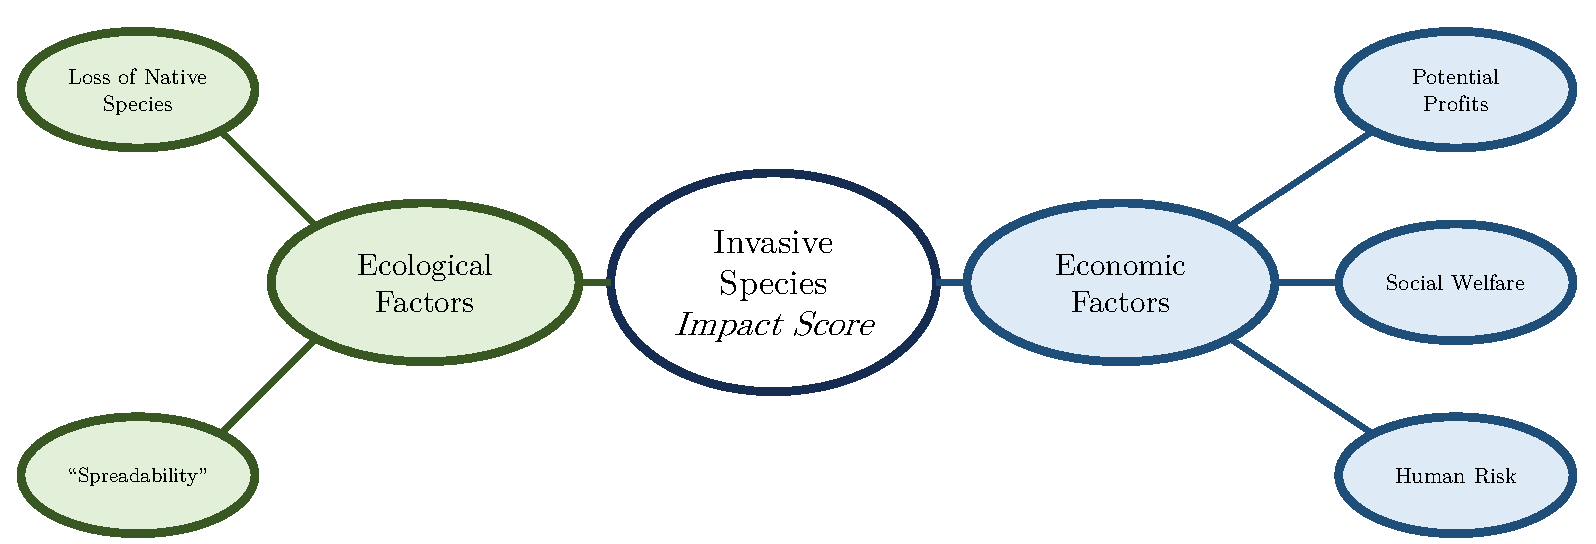
\includegraphics[scale=0.5]{figures/invasivespeciesimpactscore.pdf}
    \captionsetup{width=0.9\textwidth}
    \caption{\textbf{Overview of trade-off model.}.}
    \label{fig:invasiveimpactbrainstorm}
\end{figure}

\subsection {Assumptions}

Below, we list several core assumptions that allowed us to develop a trade-off model between ecological concerns and economic benefits. 

\begin{table}[h!]
\renewcommand{\arraystretch}{1.3}
    \begin{tabularx}{\textwidth}{lp{0.35\textwidth}X}
    \toprule
    \textbf{\#} & \textbf{Assumption} & {\centering \textbf{Justification}}  \\ \midrule
    
    \raggedright \nextassumption\label{assumption:10} & Native species prior to the introduction of a foreign species were in competitive equillibrium. & This key assumption allows us to use the Lotka-Volterra equations to compare before and after effects.\\
    
    \rowcolor{gray!15} \raggedright \nextassumption\label{assumption:11} & Foreign species follows a logistic growth with a set carrying capacity. & If a foreign species grows logistcally, we are able to create a standardized metric based on logistic regression for measuring population growth.
 \\

 \raggedright \nextassumption\label{assumption:12} & A foreign species social benefit and human health risk can be measured in dollars. & In being able to convert arbitrary ideas such as human health risk and social benefit to dollars, we are able to provide another standardized framework for these measures of impact. \\
 
    \bottomrule
    \end{tabularx}
\end{table}

\subsection{Variables}

The following list of variables summarizes the key components of our trade-off model. We will derive each of the following functions (or scores) in this section.

\begin{table}[h!]
\renewcommand{\arraystretch}{1.3}
%p{0.8\linewidth
    \begin{tabularx}{\textwidth}{p{0.25\textwidth}lX}
    \toprule
    \textbf{Variable}           & \textbf{Symbol} & \textbf{Description}  \\ \midrule
    \raggedright Native Species Population Changes & $\chi$  & Sum of proportions of changes in native species populations before and after introduction of foreign species. \\
    \rowcolor{gray!15}
    \raggedright Spreadability Rate  & $r$  & Rate of growth of foreign species by itself based on logistic regression. \\
    Economic Profit & $\pi$  & Potential profit (in dollars) made in a business centered around an foreign species. \\
    \rowcolor{gray!15} \raggedright Social Welfare Benefit& $W$   &  External social benefit not from direct harvesting of an foreign species. \\
    \raggedright Human Health Risk & $R$ & Potential risk in dollar-value cost of an foreign species to humans.\\
    \bottomrule
    \end{tabularx}
\end{table}

\subsection{Ecological Impact Score}

As a first step, we broke down our first part of the score, the ecological impact score, into three distinct categories. Regarding species to be classified as invasive, several factors are essential to consider, such as detrimental impact to native plants, the species' ability to spread (spreadability), risk to human health, and risk to native soil nutrition. Therefore, we propose an ecological impact score as a combination of these factors, none of which are dispositive. 

\subsubsection{Effects on Native Species}

To analyze the impacts of a non-native species in a new region, we need to measure the unintendend consequences in native populations. To do so, we take we used the Lotka-Volterra model (a system of differential equations) to represent the changes in population for each native species. The Volterra-Lotka model is commonly used for analyzing the population dynamics of competing species, especially in our case between nonnative and native species. 

Assuming native species are in competitive equillibrium prior to the introduction of a new non-native species (Assumption~\ref{assumption:10}), we can use a generalized set of Lotka-Volterra equations for \(n\) native species, where we can treat population growth for each species as a single vector based on the populations of other species at each time step. Furthermore, the weightings of how other native species populations affect the growth of another species can be stored in a matrix.

In mathematical terms, let there be \(n\) native species where population of a native species \(i\) where \(1 \leq i \leq n\) is denoted by \(x_i\). Therefore, the rate of change of a population \textit{in relation to} other species can be represented as 

\begin{equation}
    \frac{dx_i}{dt} = r_ix_i \left(1 - \frac{\sum\limits_{j=1}^n \alpha_{ij} x_j}{K_i}\right)
    \label{eq:lotkavolterra}
\end{equation}

where \(r_i\) is the internal growth rate of species \(i\), \(\alpha_{ij}\) is the impact of species \(j\) on species \(i\), and \(K_i\) is the carrying capacity of species \(i\). The parameters \(\alpha_{ij}\) can be combined into an \(i\) by \(i\) matrix of "interaction" parameters, therefore we denote this matrix of parameters the \textit{interaction matrix}. For the first \(n\) native species, the Lotka-Volterra equation will yield a system of \(n\) differential equations with an \(n\) by \(n\) matrix \(\alpha\). When we introduce our new foreign species, the Lotka-Volterra model will yield a system of \(n+1\) differential equations with an interaction matrix \(\alpha\) of dimensions \(n+1\) by \(n+1\) where all values \(\alpha_{ii} = 1\) for self-interaction of species.

Based on the data readily available for our use, we determined that understanding the changes in populations of 3 native species for each foreign species would be sufficient. To create a standardized score, however, we propose a native population impact score which measures \textit{ratio} of a native species prior to and after 1 year (365 days) since the introduction of a new foreign species. Therefore, let our native species impact score \(\chi\) be the sum of the ratios of native population species before and after the introduction of foreign species. Therefore, we can define our native species impact score \(\chi\) as 

\begin{equation}
    \chi = \sum_{i = 1}^n \frac{x_i {\text{ new}}}{x_i {\text{ old}}}
    \label{eq:nativepopratio}
\end{equation}

With the use of scientific software such as SciPy \cite{scipy}, we can obtain a numerical solution to this system to analyze the changes in native species population over time.

\subsubsection{Spreadability Index}

To measure spreadability, we focus on the ability of a population to regenerate and grow without competitors and with optimal access to natural resources. Regarding population growth as an logistical growth problem (See Assumptionn~\ref{assumption:11}), we develop a standardized logistic regression model to evaluate the \textit{spreadability} of a species. As most populations follow a logistic growth pattern with an ultimate environmental carrying capacity, we are able to generalize this process to most, if not all common species.

Based on historical population growth data throughout a year in an optimal setting, we can perform logistic regression on population data, such that the population data of a species can be best modeled by a function 

\begin{equation}
    N(t) = \frac{L}{1+Ce^{-rt}}
\end{equation}

for carrying capacity \(L\), constant \(C\), and proportionality constant of growth \(r\). Since \(r\) can easily describe the proportion of growth over a continuous time interval, we let our \textit{spreadability index} be the value \(r\) properly scaled by a factor of 100. So, our spreadability index can be represented as \(100r\). Therefore, we can represent the ecological impact score the sum of \(\chi\) from \(100r\) as the greater the loss in native species, the greater the ecological impact score gets.  Note that the we are looking for a lower ecological impact score of a species.

\begin{equation}
    \text{Ecological Impact Score } = 100r + \chi
    \label{eq:ecologicalimpact}
\end{equation}


\subsection{Potential Economic Potential}

Based on Assumption~\ref{assumption:12}, we primarily considered a standardized measure for analyzing the economic benefits and downfalls: monetary value. 

\subsubsection{Net Profit}

In the context of bioeconomics, a common model used to analyze the production value and potential maximum yield and profit from harvesting a specific species is called the Gordon-Schaefer Model \cite{wikipediaGordonSchaeferModel}. Gordon-Schaefer bioeconomic analysis methods can be applied whenever a species follows a logistic growth pattern, where a population levels off to some carrying capacity based on its respective environment. From the first model analyzing dandelion spread, we can see that indeed dandelions satisfy this key assumption, therefore we can apply the Gordon-Shaefer model respectively.

To find the maximum sustainable profit of an industry centered around harvesting a specific species, we can apply the microeconomic \textit{Profit Maximization Law}, where the optimal level of harvest, otherwise known as the maximum sustainable yield, can be found at the intersection of \textit{marginal revenue} and \textit{marginal cost} (MR=MC) \cite{intelligenteconomistProfitMaximization}.

In the context of a Gordon-Schaefer harvesting model, marginal revenue can be interpreted as the revenue per unit of effort in harvesting, and marginal cost can be interpreted as the cost to harvest each unit of species. As the marginal revenue decreases over time due to the Law of Diminishing Marginal Returns \cite{investopediaDiminishingMarginal}, we will calculate the optimal yield effort at the intersection of the MR and MC curve, then find that corresponding point on a \textit{Total Revenue} and \textit{Total Cost} curve to obtain the maximum profit (\(\pi\)). See Figure~\ref{fig:gordonschafer} for a visual representation of the process. Note that each species will have a Gordon Schaefer bioeconomic model calibrated to it based on industry data.

\begin{figure}[h!]
\centering
    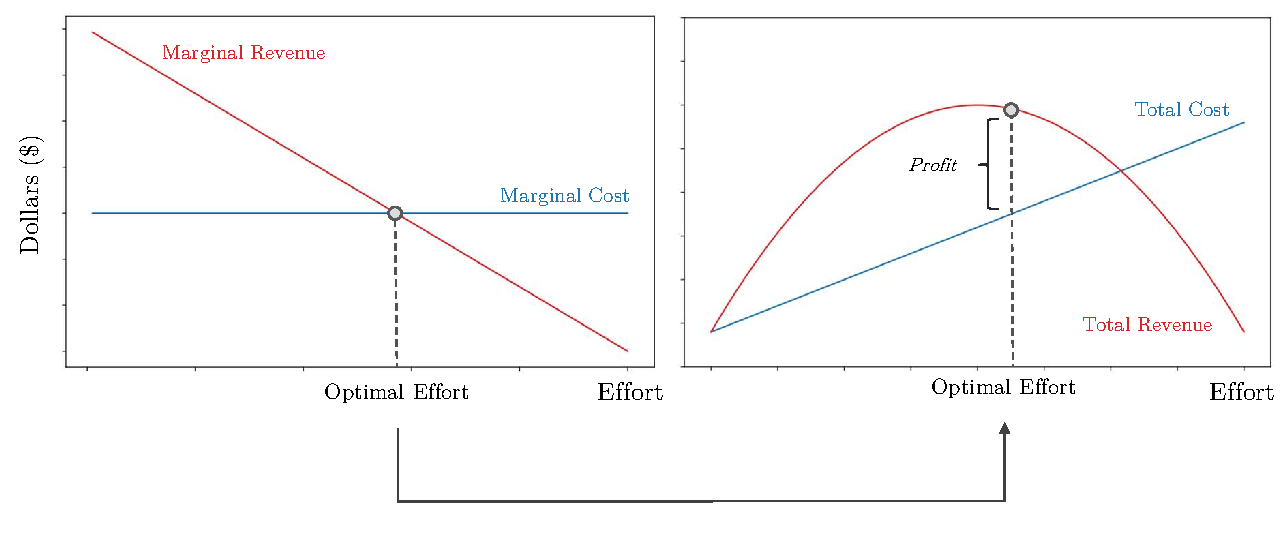
\includegraphics[scale=0.65]{figures/gordonschaefer.pdf}
    \captionsetup{width=0.9\textwidth}
    \caption{\textbf{Gordon-Schaefer model effort optimization for species harvesting.} Note that Net Profit (\(\pi\)) for the harvesting of a species can be obtained from the difference between Total Revenue and Total Cost.}
    \label{fig:gordonschafer}
\end{figure}

\subsubsection{Social Benefit}

To calculate social welfare benefit of a foreign species on society, or in more economic terms, positive externalities, we can calculate the \textit{total social welfare} received by a population surrounding the foreign species and region in question. In order to determine the explicit dollar-value benefits of social welfare, we can utilize Sen's Welfare Function (which incorporates a Gini coefficient) to model the benefits of a certain species scaled to the region's income inequalities \cite{wikipediaSocialWelfare, worldbankWorldBank}. 

Therefore, we can express the \textit{total welfare benefit} (in dollars) \(W\) as a sum of individual benefits \(Y_i\), Gini coefficient \(G\), and regional population \(n\),

\begin{equation}
    W = (1 - G) \sum_{i=1}^n Y_i
\end{equation}

\subsubsection{Human Health Risk}

To calculate human health risk as an economic factor, we analyze the average detriment a species has to humans as a sum of individual risks based on the potential amount of money lost. The sum can again be scaled similar to Sen's Welfare Function using the Gini coefficient. Data for the detrimental costs of a species to human society can be found for virtually any species, therefore, allowing us to make the assumption for generalizability.

Therefore, we express the \textit{total human risk} (in dollars) \(R\) as a sum of individual risks \(R_i\), Gini coefficient \(G\), and regional population \(n\),

\begin{equation}
    R = (1 - G) \sum_{i=1}^n R_i 
\end{equation}

Therefore, we can express the total economic benefit of a given species in a region to be the sum of economic profit and social benefit minus the human health risk.

\begin{equation}
    \text{Total Economic Benefit } = \pi + W - R
    \label{eq:economicimpact}
\end{equation}

where \(\pi\) is the maximum profit yield, \(W\) is the social welfare benefit, and \(R\) is the total human health risk. 

So, our combined foreign species trade-off score can be determined as a coordinate pair of two sub-scores: one ecological (Equation~\ref{eq:ecologicalimpact}), one economic (Equation~\ref{eq:economicimpact}), which is shown as follows.

\begin{equation}
    \text{\textbf{Impact Score} } = (\text{Ecological Score, Economic Score}) = (100r + \chi, \hspace{0.05cm} \pi + W - R)
\end{equation}